
\chapter{Introduction to Lexicalized Tree Adjoining Grammars}
\label{intro-FBLTAG}

Tree-adjoining grammar (TAG) is a formal tree rewriting system. TAG and
Lexicalized Tree-Adjoining Grammar (LTAG) have been extensively studied
both with respect to their formal properties and to their linguistic
relevance. TAG and LTAG are formally equivalent, however, from the
linguistic perspective LTAG is the system we will be concerned with in
the XTAG system. We will often use these terms TAG and LTAG
interchangeably.

The motivations for the study of LTAG are both linguistic and formal.
The elementary objects manipulated by LTAG are structured objects
(trees or directed acyclic graphs) and not strings. Using structured
objects as the elementary objects of the formal system, it is possible
to construct formalisms whose properties relate directly to the study
of strong generative capacity (i.e., structural descriptions), which is
more relevant to the linguistic descriptions than the weak generative
capacity (sets of strings).

Each grammar formalism specifies a domain of locality, i.e., a domain
over which various dependencies (syntactic and semantic) can be
specified. It turns out that the various properties of a formalism
(syntactic, semantic, computational, and even psycholinguistic) follow,
to a large extent, from the initial specification of the domain of
locality.

\begin{figure*}[ht] 
\begin{center}
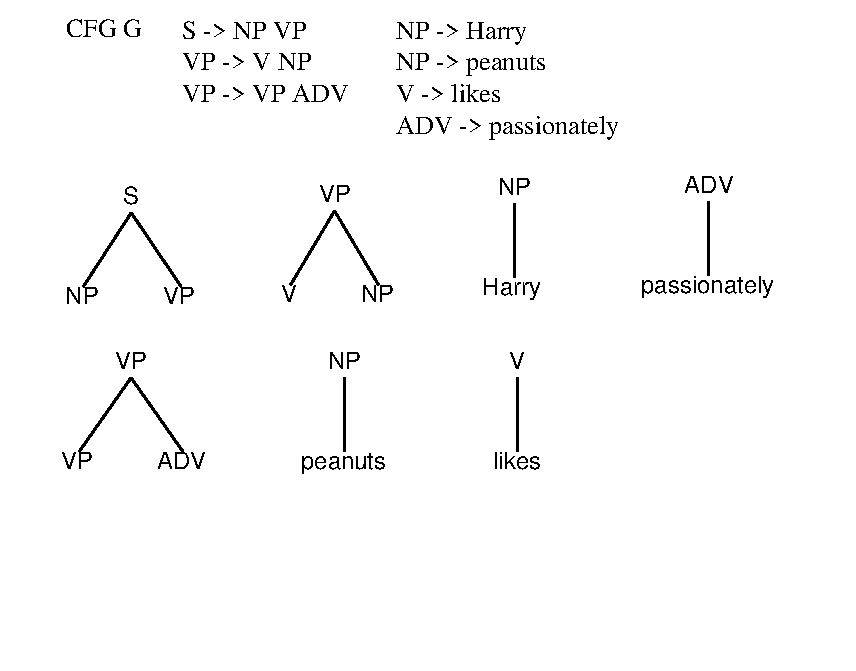
\includegraphics[height=3in]{ps/intro-files/cfg-locality.eps}
\caption{\label{cfg} Domain of locality of a context-free grammar}
\end{center}
\end{figure*}

\subsection{Domain of locality of CFGs} 

In a context-free grammar (CFG) the domain of locality is the one level
tree corresponding to a rule in a CFG (Fig.~\ref{cfg}). It is easily
seen that the arguments of a predicate (for example, the two arguments
of {\it likes}) are not in the same local domain. The two arguments are
distributed over the two rules (two domains of locality)-- $S
\rightarrow NP \ VP$ and $VP \rightarrow V \ NP$. They can be brought
together by introducing a rule $S \rightarrow NP \ V \ VP $. However,
then the structure provided by the VP node is lost. We should also note
here that not every rule (domain) in the CFG in (Fig.~\ref{cfg}) is
lexicalized. The three rules on the right are lexicalized, i.e., they
have a lexical anchor. The rules on the right are not lexicalized. The
second and the third rules on the left are almost lexicalized, in the
sense that they each have a preterminal category ($V$ in the second
rule and $ADV$ in the third rule), i.e., by replacing $V$ by {\it
likes} and $ADV$ by {\it passionately} these two rules will become
lexicalized. However, the first rule on the left ($S \rightarrow NP
\ VP$) cannot be lexicalized. Can a CFG be lexicalized, i.e., given a
CFG, $G$, can we construct another CFG, $G'$, such that every rule in
$G'$ is lexicalized and $T(G)$, the set of (sentential) trees (i.e.,
the tree language of $G$) is the same as the tree language $T(G')$ of
$G'$? It can be shown that this is not the case \cite{joshischabes96}.
Of course, if we require that only the string languages of $G$ and $G'$
be the same (i.e., they are weakly equivalent) then any CFG can be
lexicalized. This follows from the fact that any CFG can be put in the
Greibach normal form where each rule is of the form $ A \rightarrow w
\ B1 \ B2 \ ... \ Bn$ where $w$ is a lexical item and the $B's$ are
nonterminals. The lexicalization we are interested in requires the
tree languages (i.e., the set of structural descriptions) be the same,
i.e., we are interested in the `strong' lexicalization. To summarize, a
CFG cannot be strongly lexicalized by a CFG. This follows from the fact
that the domain of locality of CFG is a one level tree corresponding to
a rule in the grammar. Note that there are two issues we are concerned
with here-- lexicalization of each elementary domain and the
encapsulation of the arguments of the lexical anchor in the elementary
domain of locality. The second issue is independent of the first issue.
From the mathematical point of view the first issue, i.e., the
lexicalization of the elementary domains of locality is the crucial
one. We can obtain strong lexicalization without satisfying the
requirement specified in the second issue (encapsulation of the
arguments of the lexical anchor). Of course, from the linguistic point
view the second issue is very crucial. What this means is that among
all possible strong lexicalizations we should choose only those that
meet the requirements of the second issue. In implementing a grammar in
the XTAG system we will assume that we always make such a choice.


\begin{figure*}[ht] 
\begin{center}
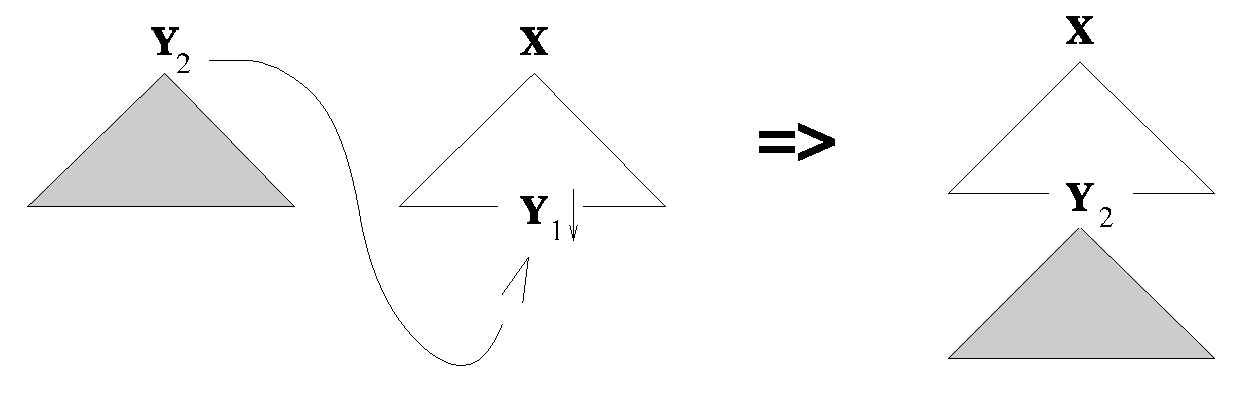
\includegraphics[height=1.5in]{ps/intro-files/schematic-subst2.eps}
\caption{\label{substitution} Substitution}
\end{center}
\end{figure*}

\begin{figure*}[ht] 
\begin{center}
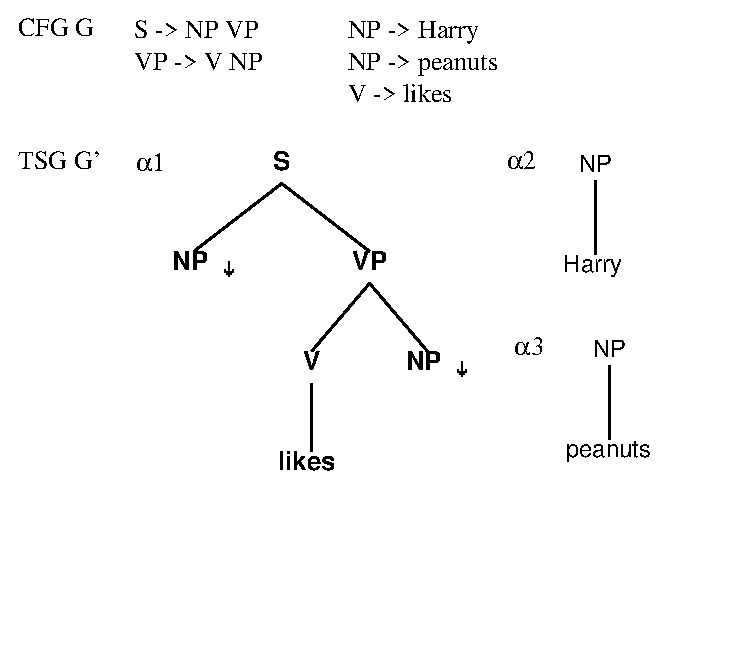
\includegraphics[height=2.5in]{ps/intro-files/treesubst.eps}
\caption{\label{tsg} Tree substitution grammar}
\end{center}
\end{figure*}

\subsection{Lexicalization of CFGs}

Now we can ask the following question. Can we strongly lexicalize a
CFG by a grammar with a larger domain of locality?
Fig.~\ref{substitution} and Fig.~\ref{tsg} show a tree substitution
grammar where the elementary objects (building blocks) are the three
trees in Fig.~\ref{tsg} and the combining operation is the tree
substitution operation shown in Fig.~\ref{substitution}. Note that
each tree in the tree substitution grammar (TSG), $G'$ is lexicalized,
i.e., it has a lexical anchor. It is easily seen that $G'$ indeed
strongly lexicalizes $G$. However, TSG's fail to strongly lexicalize
CFG's in general. We show this by an example. Consider the CFG, $G$,
in Fig.~\ref{tsg2} and a proposed TSG, $G'$. It is easily seen that
although $G$ and $G'$ are weakly equivalent they are not strongly
equivalent. In $G'$, suppose we start with the tree $\alpha_1$ then by
repeated substitutions of trees in $G'$ (a node marked with a vertical
arrow denotes a substitution site) we can grow the right side of
$\alpha_1$ as much as we want but we cannot grow the left
side. Similarly for $\alpha_2$ we can grow the left side as much as we
want but not the right side. However, trees in $G$ can grow on both
sides. Hence, the TSG, $G'$, cannot strongly lexicalize the CFG, $G$
\cite{joshischabes96}.


\begin{figure*}[ht] 
\begin{center}
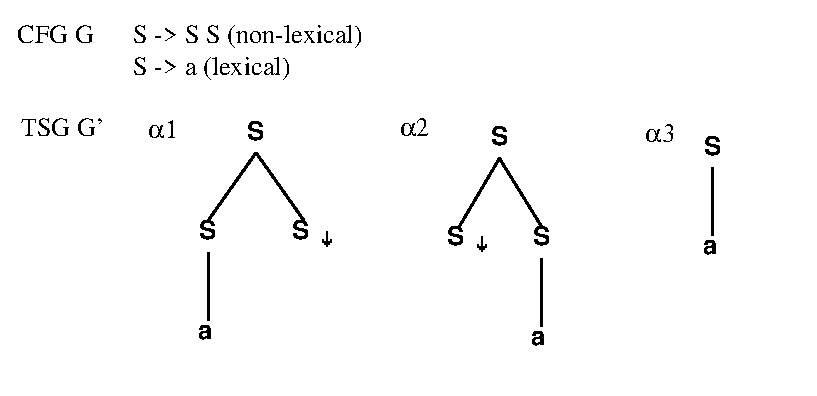
\includegraphics[height=1.8in]{ps/intro-files/treesubst-rec.eps}
\caption{\label{tsg2} A tree substitution grammar}
\end{center}
\end{figure*}


\begin{figure*}[ht] 
\begin{center}
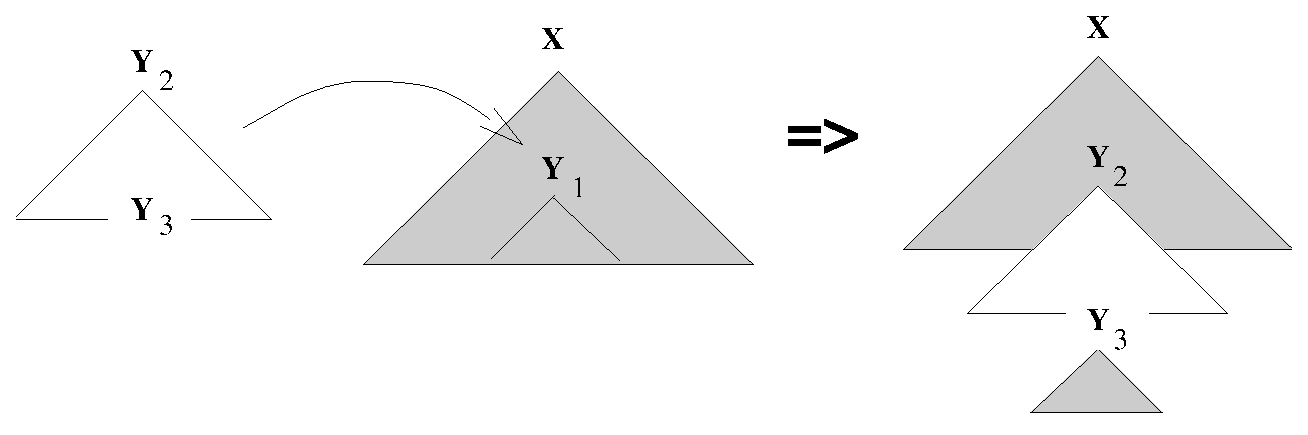
\includegraphics[height=1.5in]{ps/intro-files/schematic-adjunction2.eps}
\caption{\label{adjunction} Adjoining}
\end{center}
\end{figure*}

\begin{figure*}[ht] 
\begin{center}
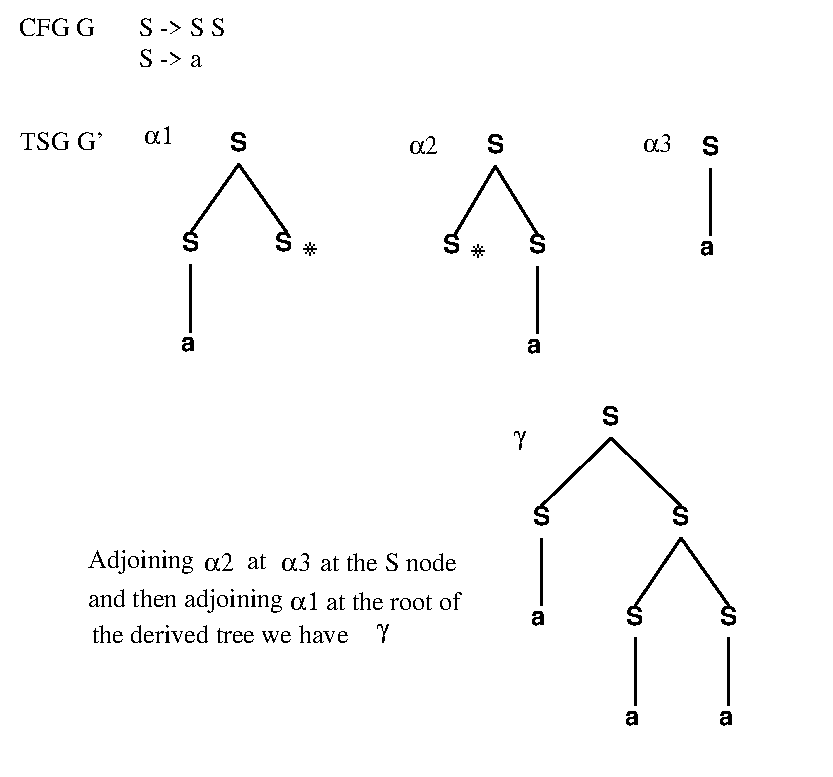
\includegraphics[height=3in]{ps/intro-files/adj-arise.eps}
\caption{\label{tsg-adj} Adjoining arises out of lexicalization}
\end{center}
\end{figure*}

We now introduce a new operation called `adjoining' as shown in
Fig.~\ref{adjunction}. Adjoining involves splicing (inserting) one
tree into another. More specifically, a tree $\beta$ as shown in
Fig.~\ref{adjunction} is inserted (adjoined) into the tree $\alpha$ at
the node $X$ resulting in the tree $\gamma$. The tree $\beta$, called
an auxiliary tree, has a special form. The root node is labeled with a
nonterminal, say $X$ and on the frontier there is also a node labeled
$X$ called the foot node (marked with *). There could be other nodes
(terminal or nonterminal) nodes on the frontier of $\beta$, the
nonterminal nodes will be marked as substitution sites (with a
vertical arrow). Thus if there is another occurrence of $X$ (other
than the foot node marked with *) on the frontier of $\beta$ it will
be marked with the vertical arrow and that will be a substitution
site. Given this specification, adjoining $\beta$ to $\alpha$ at the
node $X$ in $\alpha$ is uniquely defined. Adjoining can also be seen
as a pair of substitutions as follows: The subtree at $X$ in $\alpha$
is detached, $\beta$ is substituted at $X$ and the detached subtree is
then substituted at the foot node of $\beta$. A tree substitution
grammar when augmented with the adjoining operation is called a
tree-adjoining grammar (lexicalized tree-adjoining grammar because
each elementary tree is lexically anchored). In short, LTAG consists
of a finite set of elementary trees, each lexicalized with at least
one lexical anchor. The elementary trees are either initial or
auxiliary trees. Auxiliary trees have been defined already. Initial
trees are those for which all nonterminal nodes on the frontier are
substitution nodes. It can be shown that any CFG can be strongly
lexicalized by an LTAG~\cite{joshischabes96}.

In Fig.~\ref{tsg-adj} we show a TSG, $G'$, augmented by the operation
of adjoining, which strongly lexicalizes the CFG, $G$. Note that the
LTAG looks the same as the TSG considered in Fig.~\ref{tsg2}. However,
now trees $\alpha_1$ and $\alpha_2$ are auxiliary trees (marked with
*) that can participate in adjoining. Since adjoining can insert a
tree in the interior of another tree it is possible to grow both sides
of the tree $\alpha_1$ and tree $\alpha_2$, which was not possible
earlier with substitution alone. In summary, we have shown that by
increasing the domain of locality we have achieved the following: (1)
lexicalized each elementary domain, (2) introduced an operation of
adjoining, which would not be possible without the increased domain of
locality (note that with one level trees as elementary domains
adjoining becomes the same as substitution since there are no interior
nodes to be operated upon), and (3) achieved strong lexicalization of
CFGs.


\begin{figure*}[ht] 
\begin{center}
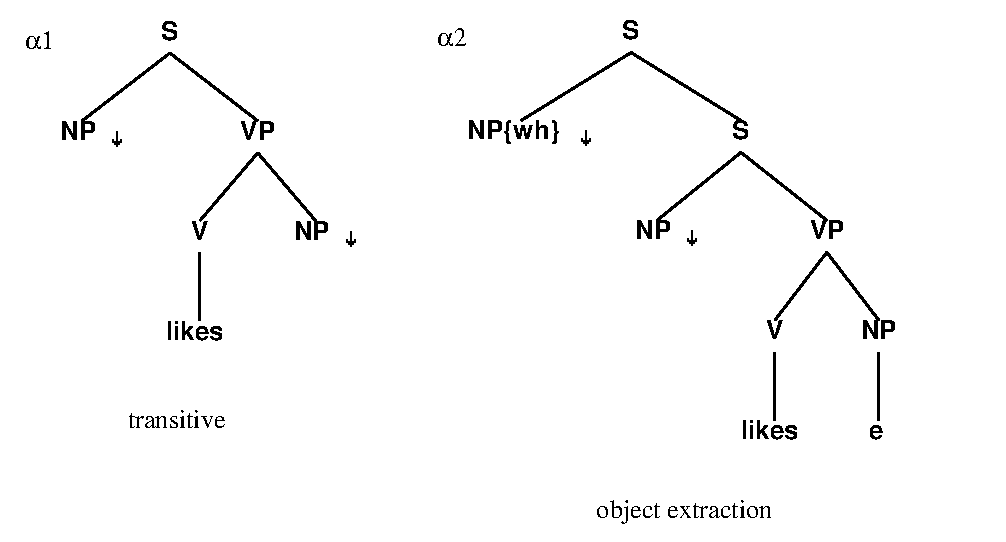
\includegraphics[height=2in]{ps/intro-files/likes-ex.eps}
\caption{\label{trees-likes} LTAG: Elementary trees for {\it likes}}
\end{center}
\end{figure*}

\begin{figure*}[ht] 
\begin{center}
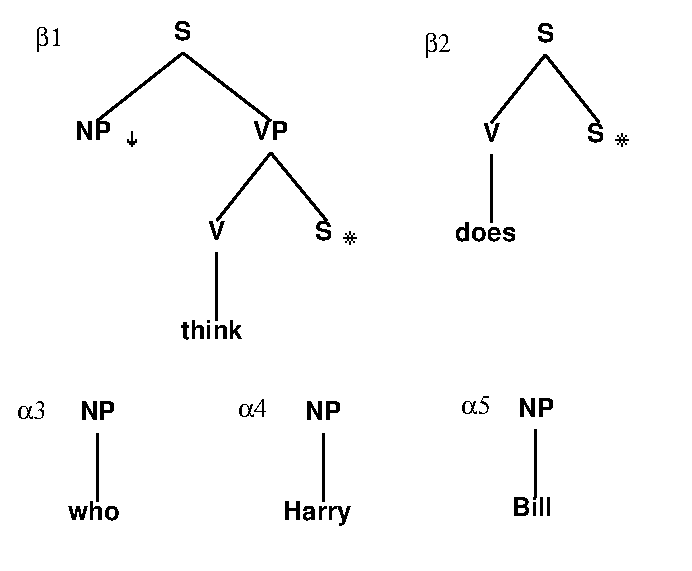
\includegraphics[height=2in]{ps/intro-files/ltag-sampletrees.eps}
\caption{\label{more-trees} LTAG: Sample elementary trees}
\end{center}
\end{figure*}

\subsection{Lexicalized tree-adjoining grammars}

Rather than giving formal definitions for LTAG and derivations in LTAG
we will give a simple example to illustrate some key aspects of
LTAG. We show some elementary trees of a toy LTAG grammar of
English. Fig.~\ref{trees-likes} shows two elementary trees for a verb
such as {\it likes}. The tree $\alpha_1$ is anchored on {\it likes}
and encapsulates the two arguments of the verb. The tree $\alpha_2$
corresponds to the object extraction construction. Since we need to
encapsulate all the arguments of the verb in each elementary tree for
{\it likes}, for the object extraction construction, for example, we
need to make the elementary tree associated with {\it likes} large
enough so that the extracted argument is in the same elementary
domain. Thus, in principle, for each `minimal' construction in which
{\it likes} can appear (for example, subject extraction,
topicalization, subject relative, object relative, passive, etc.)
there will be an elementary tree associated with that construction. By
`minimal' we mean when all recursion has been factored away. This
factoring of recursion away from the domain over which the
dependencies have to be specified is a crucial aspect of LTAGs as they
are used in linguistic descriptions. This factoring allows all
dependencies to be localized in the elementary domains. In this sense,
there will, therefore, be no long distance dependencies as such. They
will all be local and will become long distance on account of the
composition operations, especially adjoining.


\begin{figure*}[ht] 
\begin{center}
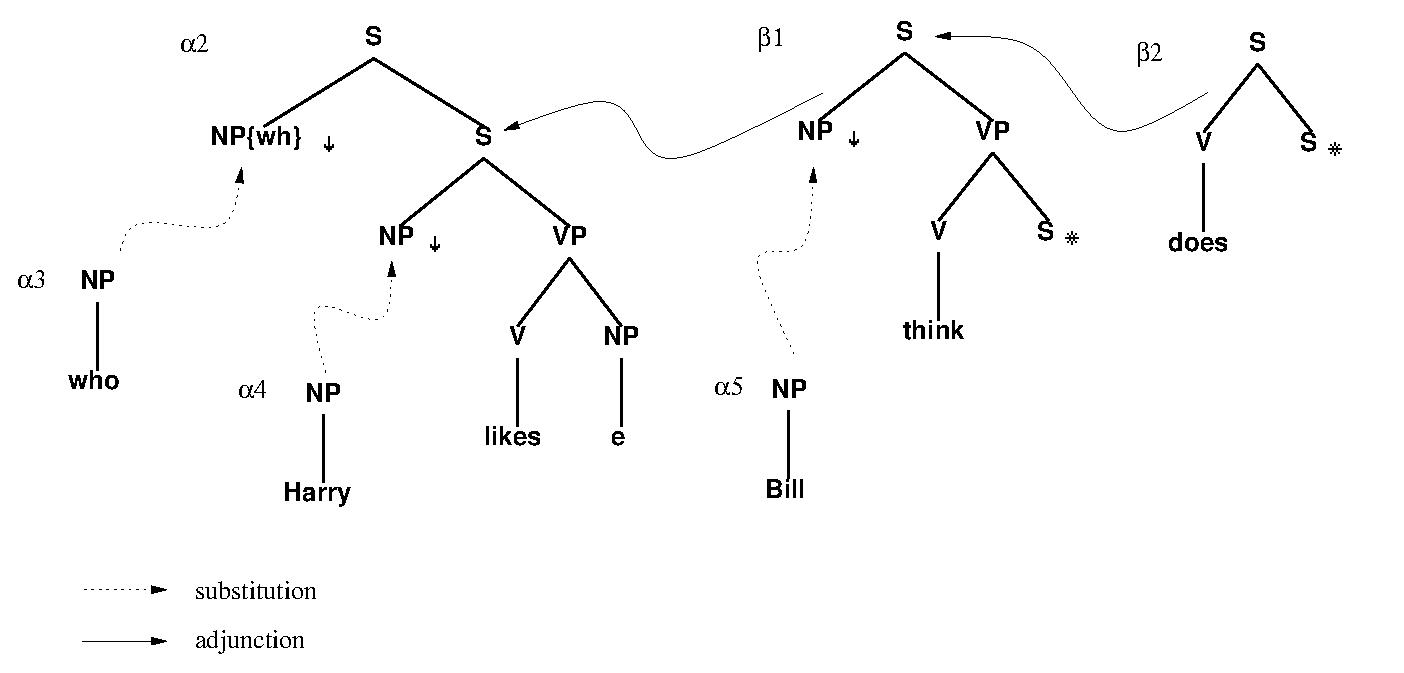
\includegraphics[height=2.5in]{ps/intro-files/ltag-derivation.eps}
\caption{\label{ltag-derivation} LTAG derivation for {\it who does Bill think Harry likes}}
\end{center}
\end{figure*}

Fig.~\ref{more-trees} shows some additional trees. Trees $\alpha_3$,
$\alpha_4$, and $\alpha_5$ are initial trees and trees $\beta_1$ and
$\beta_2$ are auxiliary trees with foot nodes marked with *. A
derivation using the trees in Fig.~\ref{more-trees} is shown in
Fig.~\ref{ltag-derivation}. The trees for {\it who} and {\it Harry}
are substituted in the tree for {\it likes} at the respective $NP$
nodes, the tree for {\it Bill} is substituted in the tree for {\it
think} at the $NP$ node, the tree for {\it does} is adjoined to the
root node of the tree for {\it think} tree (adjoining at the root node
is a special case of adjoining), and finally the derived auxiliary
tree (after adjoining $\beta_2$ to $\beta_1$) is adjoined to the
indicated interior $S$ node of the tree $\alpha_2$. This derivation
results in the derived tree for {\it who does Bill think Harry likes}
as shown in Fig.~\ref{derived-tree}. Note that the dependency between
{\it who} and the complement $NP$ in $\alpha_2$ (local to that tree)
has been stretched in the derived tree in
Fig.~\ref{derived-tree}. This tree is the conventional tree associated
with the sentence.


\begin{figure*}[ht] 
\begin{center}
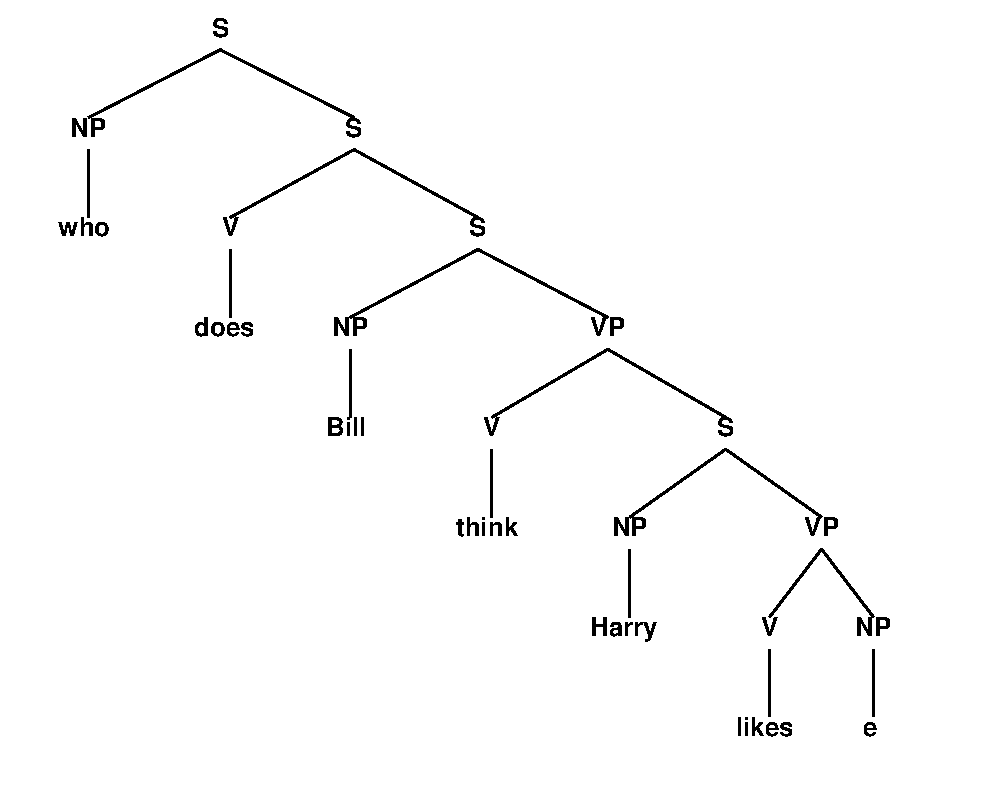
\includegraphics[height=2.5in]{ps/intro-files/ltag-derived-tree.eps}
\caption{\label{derived-tree} LTAG derived tree for {\it who does Bill think Harry likes}}
\end{center}
\end{figure*}


However, in LTAG there is also a derivation tree, the tree that
records the history of composition of the elementary trees associated
with the lexical items in the sentence. This derivation tree is shown
in Fig.~\ref{ltag-derivation-tree}. The nodes of the tree are labeled
by the tree labels such as $\alpha_2$ together with the lexical
anchor\footnote{The derivation trees of LTAG have a close relationship
to the dependency trees, although there are some crucial differences;
however, the semantic dependencies are the same.}.  The derivation
tree is the crucial derivation structure for LTAG. We can obviously
build the derived tree from the derivation tree. For semantic
computation the derivation tree (and not the derived tree) is the
crucial object. Compositional semantics is defined on the derivation
tree. The idea is that for each elementary tree there is a semantic
representation associated with it and these representations are
composed using the derivation tree. Since the semantic representation
for each elementary tree is directly associated with the tree there is
no need to reproduce necessarily the internal hierarchy in the
elementary tree in the semantic
representation~\cite{joshi99:_compos_ltag}. This allows the so-called
`flat' semantic representation as well as helps in dealing with some
non-compositional aspects as in the case of rigid and flexible idioms.


\begin{figure*}[ht] 
\begin{center}
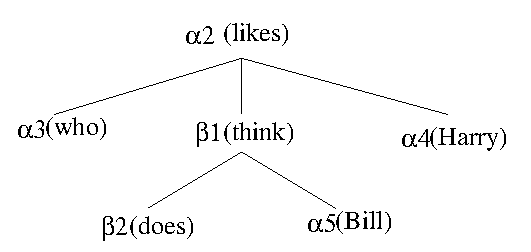
\includegraphics[height=1.5in]{ps/intro-files/ltag-derivation-tree.eps}
\caption{\label{ltag-derivation-tree} LTAG derivation tree}
\end{center}
\end{figure*}

\section{Some important properties of LTAG}

The two key properties of LTAG are (1) extended domain of locality
(EDL) (for example, as compared to CFG), which allows (2) factoring
recursion from the domain of dependencies (FRD), thus making all
dependencies local. All other properties of LTAG (mathematical,
linguistic, and even psycholinguistic) follow from EDL and FRD. TAGs
(LTAGs) belong to the so-called class of mildly context-sensitive
grammars~\cite{joshi85}. CFL's are properly contained in the class of
languages of LTAG, which in turn are properly contained in the class
of context-sensitive languages. There is a machine characterization of
TAG (LTAG), called embedded pushdown automaton (EPDA)~\cite{vijay87},
i.e., for every TAG language there is an EPDA which corresponds to
this (and only this) language and the language accepted by any EPDA is
a TAG language. EPDAs have been used to model some psycholinguistic
phenomena, for example, processing crossed dependencies and nested
dependencies have been in discussed in~\cite{joshi90}. With respect to
formal properties, the class of TAG languages enjoys all the important
properties of CFLs, including polynomial parsing (with complexity
$O(n^{6}$)).

\section{Unification-based features}

In the XTAG system, each node in each LTAG tree is decorated with two
feature structures (top and bottom feature structures), in contrast to
the CFG based feature structure grammars, because adjoining can augment
a tree internally, while in a CFG based grammar a tree can be augmented
only at the frontier. It is possible to define adjoining and
substitution (as it is done in the XTAG system) in terms of appropriate
unifications of the top and bottom feature structures. Because of FRD
(factoring recursion from the domain of dependencies), there is no
recursion in the feature structures. Therefore, in principle, feature
structures can be eliminated. However, they are crucial for linguistic
descriptions. Constraints on substitution and adjoining are modeled via
these feature structures~\cite{vijay87}. This method of manipulating
feature structures is a direct consequence of the extended domain of
locality of LTAG.

In a unification framework, a feature structure is associated with each
node in an elementary tree.  This feature structure contains
information about how the node interacts with other nodes in the tree.
It consists of a top part, which generally contains information
relating to the supernode, and a bottom part, which generally contains
information relating to the subnode.  Substitution nodes, however, have
only the top features, since the tree substituting in logically carries
the bottom features.

\begin{figure}[htb]
\centering
\begin{tabular}{c}
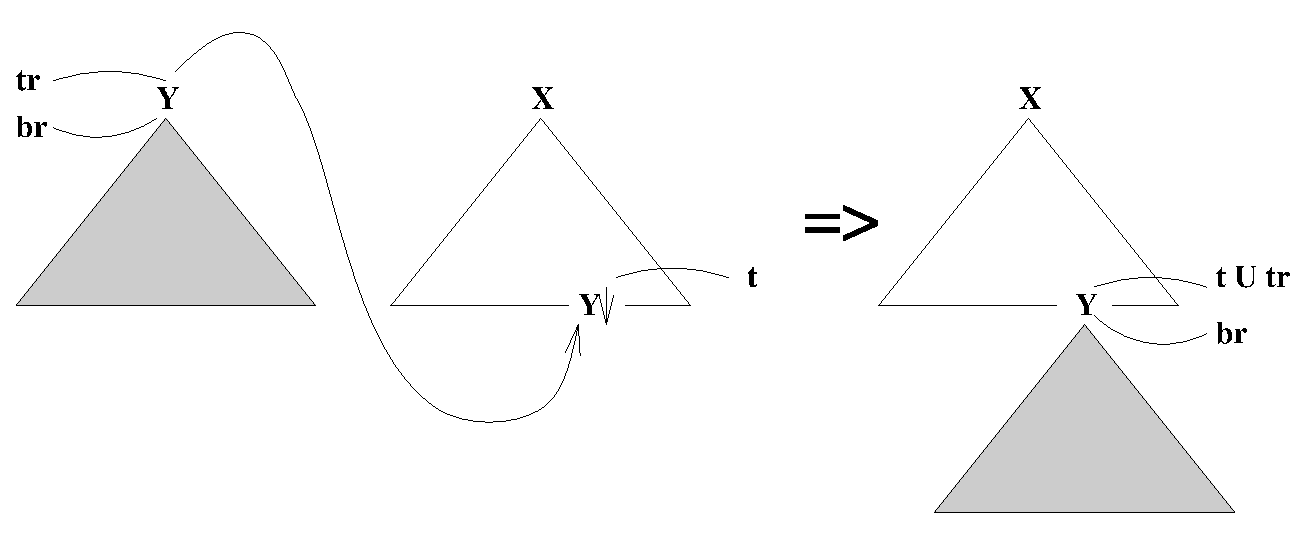
\includegraphics[height=1.5in]{ps/intro-files/schematic-feat-subst.eps}
\end{tabular}
\caption{Substitution in FB-LTAG}
\label{subst-fig}
\end{figure}

The notions of substitution and adjunction must be augmented to fit
within this new framework.  The feature structure of a new node created
by substitution inherits the union of the features of the original
nodes.  The top feature of the new node is the union of the top
features of the two original nodes, while the bottom feature of the new
node is simply the bottom feature of the top node of the substituting
tree (since the substitution node has no bottom feature).  Figure
\ref{subst-fig}\footnote{abbreviations in the figure:  t$=$top feature
structure, tr$=$top feature structure of the root, br$=$bottom feature
structure of the root, U$=$unification} shows this more clearly.

\begin{figure}[htb]
\centering
\begin{tabular}{c}
\hspace{0.65in}
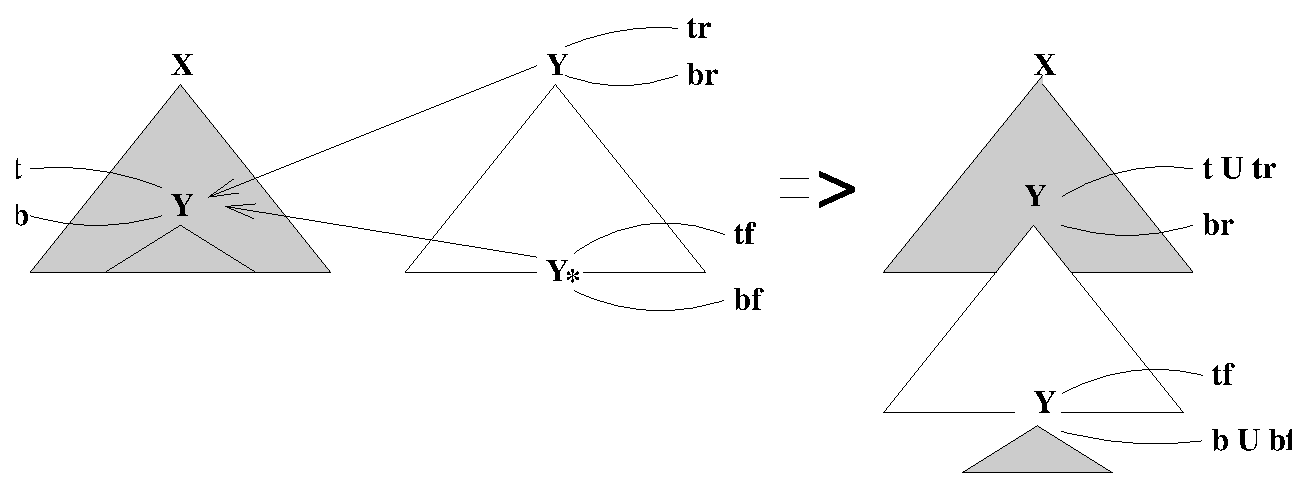
\includegraphics[height=1.5in]{ps/intro-files/schematic-feat-adjunction.eps}
\end{tabular}
\caption{Adjunction in FB-LTAG}
\label{adjunct-fig}
\end{figure}

Adjunction is only slightly more complicated.  The node being adjoined into
splits, and its top feature unifies with the top feature of the root
adjoining node, while its bottom feature unifies with the bottom feature of the
foot adjoining node.  Again, this is easier shown graphically, as in Figure
\ref{adjunct-fig}\footnote{abbreviations in the figure: t$=$top
feature structure, b$=$bottom feature structure, tr$=$top feature
structure of the root, br$=$bottom feature structure of the root,
tf$=$top feature structure of the foot, bf$=$bottom feature structure
of the foot, U$=$unification}.

\begin{figure}[htbp]
\centering
\begin{tabular}{ccc}
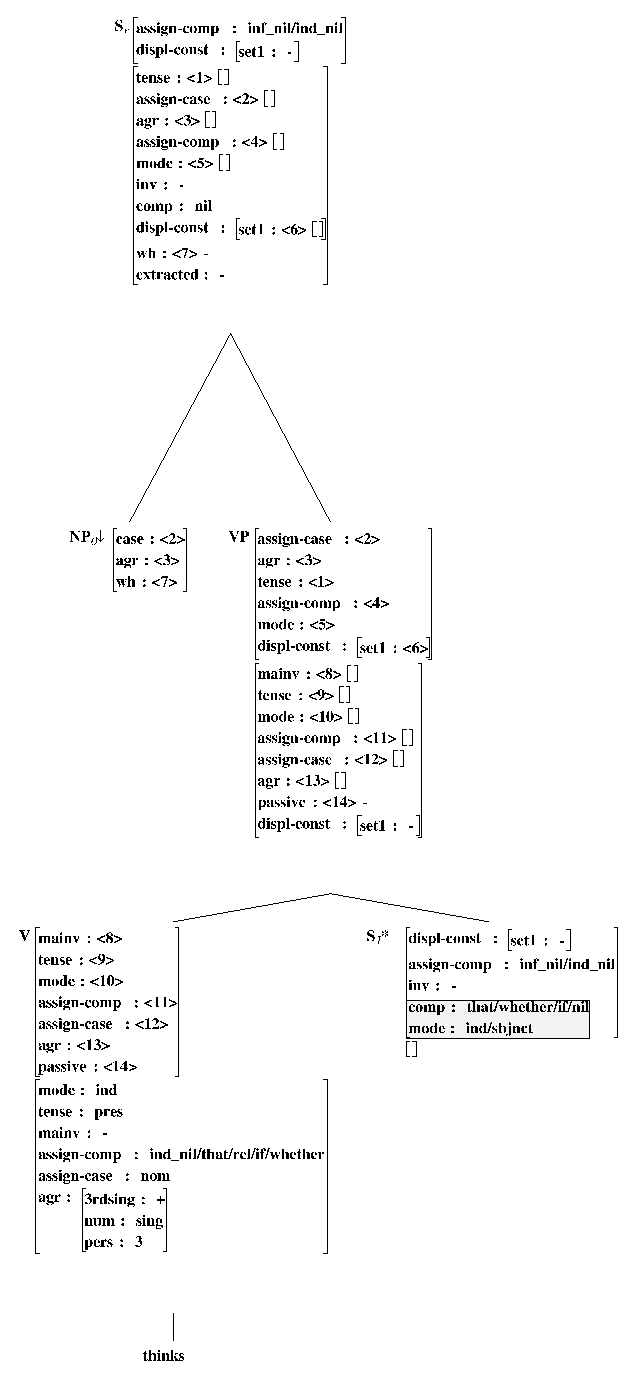
\includegraphics[height=4.5in]{ps/intro-files/think-feat.eps}  &
\hspace{0.6in}
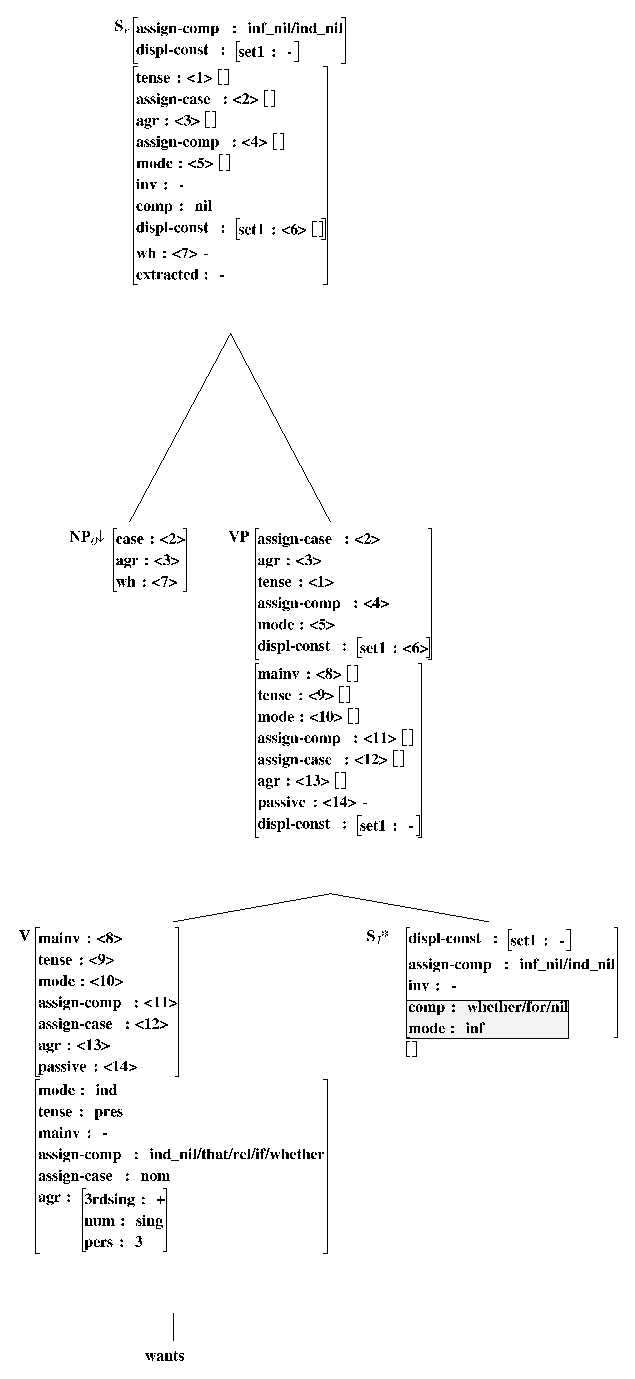
\includegraphics[height=4.5in]{ps/intro-files/want-feat.eps} \\
{\it think} tree&{\it want} tree\\
\end{tabular}\\
\caption {Lexicalized Elementary Trees with Features}
\label {lex-with-features}
\label{2;Tnx0Vs1}
\end{figure}


The embedding of the TAG formalism in a unification framework allows
us to dynamically specify local constraints that would have otherwise
had to have been made statically within the trees.  Constraints that
verbs make on their complements, for instance, can be implemented
through the feature structures.  The notions of Obligatory and
Selective Adjunction, crucial to the formation of lexicalized
grammars, can also be handled through the use of
features.\footnote{The remaining constraint, Null Adjunction (NA),
must still be specified directly on a node.} Perhaps more important to
developing a grammar, though, is that the trees can serve as a
schemata to be instantiated with lexical-specific features when an
anchor is associated with the tree.  To illustrate this, Figure
\ref{lex-with-features} shows the same tree lexicalized with two
different verbs, each of which instantiates the features of the tree
according to its lexical selectional restrictions.

In Figure \ref{lex-with-features}, the lexical item {\it thinks} takes an
indicative sentential complement, as in the sentence {\it John thinks that Mary
loves Sally}.  {\it Want} takes a sentential complement as well, but an
infinitive one, as in {\it John wants to love Mary}.  This distinction is
easily captured in the features and passed to other nodes to constrain which
trees this tree can adjoin into, both cutting down the number of separate trees
needed and enforcing conceptual Selective Adjunctions (SA).

\section{Some related systems}

{\bf Categorial Grammars:} Categories assigned to lexical items in a
categorial grammar framework do encapsulate the arguments of the
lexical anchor. It is of interest to see how the basic ideas in LTAG
could be incorporated in a categorial framework. The idea is not to
translate LTAG into a categorial grammar but rather construct a
categorial system with properties similar to LTAG. This is achieved by
associating partial proof trees with lexical items. These partial
proof trees are obtained by starting with the type assignment for a
lexical item as specified by a categorial grammar and then `unfolding'
it by using certain categorial inference rules such as function
application. This unfolding is done until the slots for the arguments
of the lexical anchor are exposed. We thus have a finite collection of
partial proof trees (lexicalized, of course) which serve as the
building blocks of our system (analogous to the finite set of
elementary trees in LTAG). These proof trees are then combined by
universal categorial inference rules in terms of cuts. Informally
speaking, the proof trees are hooked up by linking the conclusion
nodes of one tree to the assumption nodes of another tree. For a
further discussion of such systems and their relationship to LTAG can
be found in \cite{JoshiKulick97,joshi99:_proof_trees}.

{\bf From sentence structure to discourse structure:} Using the
insights from LTAG a structural and presuppositional a ccount of local
discourse structure has been presented
in~\cite{webber99:_discourse_tag}. The idea is to start the analysis
of discourse in the same way as one starts the analysis of a clause,
looking at how its syntax and semantics project from the lexicon. This
is complementary to the issue of discourse pragmatics --how these
small syntactic units of discourse are used in achieving communicative
intentions --and to the other discourse processes that provide
additional organizational overlays on these units. A key feature of
this approach is that semantic discourse relations are associated with
syntactic structures and anaphoric links, and that the properties of
the two are (not surprisingly) different. Together they allow more
complex semantics to be conveyed through simpler structures.

{\bf Phrase structure composition and syntactic dependencies:}
\cite{frank00:_tag_book} presents a comprehensive perspective on phrase
structure composition and syntactic dependencies in a TAG-based
grammatical architecture and compares it to the minimalist framework,
showing that a number of stipulative and problematic aspects of that
theory can be eliminated.



\section{Summary}

The domain of locality of a grammar formalism, i.e., the domain over
which various dependencies can be specified determines to a large
extent the syntactic, semantic, computational, and even
psycholinguistic properties of the formalism. From this perspective the
extended domain of Lexicalized Tree-Adjoining Grammars (LTAG) --
extended as compared to the domain of locality of CFGs, for example --
was explored. This extended domain is achieved by specifying the
elementary objects of the grammar as structured objects instead of
strings, together with two universal combining operations (substitution
and adjoining). This perspective allows us to study directly many
aspects of strong generative capacity which are more useful for
linguistic description.

